\documentclass[12pt,a4paper]{report}
\usepackage[utf8]{inputenc}
\usepackage{amsmath}
\usepackage{amsfonts}
\usepackage{amssymb}
\usepackage{makeidx}
\usepackage{graphicx}
\usepackage{algorithm,listings}
\usepackage{algpseudocode}

\usepackage[left=4cm,right=2cm,top=3cm,bottom=3cm]{geometry}
\newcommand{\mySpace}{0.6cm}
\usepackage{tikz}
\usetikzlibrary{shapes,arrows,positioning}
\renewcommand{\contentsname}{\centering Contents}
\usepackage{hyperref}
\begin{document}
\clearpage
	\newgeometry{left=2cm, right=2cm, top=3cm, bottom=3cm}
	\begin{titlepage}

    \centering
    {\Huge Gesture-Nav: Hand-Controlled Virtual Mouse \fontsize{24}{28.8}\selectfont \fontfamily{ptm}\selectfont}\\
\vspace{\mySpace}
%	\begin{center}
 %   		{\fontsize{24}{28.8}\selectfont  {Gesture-Nav: Hand-Controlled Virtual Mouse}}
%	\end{center}
    \large \textit{By}\\
\vspace{\mySpace}
    {\Large TAMAL MALLIK ( CSE21099 / 759 ) \\
    \vspace{0.1cm}
    AVISHEK MONDAL ( CSE21019 / 679 ) \\
    \vspace{0.1cm}
    SOUVIK BAIDYA ( CSE21088  / 748 ) \\
    \fontsize{18}{22}\selectfont \fontfamily{ptm}\selectfont
\vspace{\mySpace}}
    \begin{center}
        
\includegraphics[width=0.5\textwidth]{iiitk_logo} %img
    \end{center}
    {\Large \textit{Bachelor Thesis submitted to}\\
    \vspace{\mySpace}
    Indian Institute of Information Technology Kalyani \\ \vspace{\mySpace}
	 \textit{for the partial fulfillment of the degree of}\\ \vspace{\mySpace}

{\bfseries %bolding
	 Bachelor of Technology \\
	 in \\
	 Computer Science and Engineering\\
\vspace{\mySpace}
	  November, 2023 \fontsize{18}{22}}\selectfont \fontfamily{ptm}\selectfont}
    \vspace*{\fill}
\end{titlepage}
\restoregeometry


%	\author{Tamal Mallick , Avishek Mondal, Souvik Baidya}
%	\title{GestureNav: Hand-Controlled Virtual Mouse }
%	\maketitle
%	GestureNav: Hand Controlled Virtual Mouse
%
	\newpage
	\pagenumbering{roman}
	\chapter*{\centering Certificate}
\label{sec:engack}
This is to certify that the synopsis entitled \textbf{Gesture-Nav: Hand-Controlled Virtual Mouse} is being submitted by Tamal Mallick,
 (\textbf{Enrollment No.: CSE/21099\\/759}), Avishek Mondal (\textbf{Enrollment No.: CSE21019/679} and Souvik Baidya (\textbf{Enrollment No.: CSE21088/748}, B.Tech., Indian Institute of Information Technology Kalyani, India, for the partial fulfillment of the requirements for the registration of the degree of Bachelor of Technology is an original research work carried by them under my supervision. The synopsis has fulfilled all the requirements as per the regulation of IIIT Kalyani and in my opinion, has reached the standards needed for submission. The works, techniques, and results presented have not been submitted to any other university or Institute for the award of any other degree or diploma.
\\
\\
\\
\\
\\
\\
\\
\\
\textbf{Dr. Anirban Lakshman}  \\ 
$Assistant Professor \\  
Department of Mathematics\\
Indian Institute of Information Technology Kalyani\\
Kalyani-741235, W.B., India.
$
\cleardoublepage



	\chapter*{\centering Declaration}
\label{sec:engack}
We hereby declare that the work being submitted in this thesis entitled,\textbf{"Gesture-Nav: Hand-Controlled Virtual Mouse"}, submitted to Indian Institute of Information Technology, Kalyani in partial fulfillment for the award of the degree of Bachelor of Technology in Computer Science and Engineering during the period from July, 2023 to November 2023 under the supervision of Dr. Anirban Lakshman, Department of Computer Science and Engineering, Indian Institute of Information Technology Kalyani, West Bengal 741235, India, does not contain any classified information. 
\\
\\
\\
\\
\\
\\
\\
$
\\
\textbf{Tamal Mallick} \\
Enrollment No.: CSE/21099/759\\
Indian Institute of Information Technology Kalyani\\
Kalyani - 741235, W.B., India.
\\
\\
\\
\\
\textbf{Avishek Mondal}\\
Enrollment No.: CSE/21019/679\\
Indian Institute of Information Technology Kalyani\\
Kalyani - 741235, W.B., India.
\\
\\
\\
\\
\textbf{Souvik Baidya}\\
Enrollment No.: CSE21088/748\\
Indian Institute of Information Technology Kalyani\\
Kalyani - 741235, W.B., India.
$

\cleardoublepage
	
			\newpage
			\chapter*{\centering Acknowledgement}
We hereby acknowledge our deep sense of gratitude to our supervisor Dr. Anirban Lakshman, Department of Mathematics, Indian Institute of Information Technology Kalyani, for providing us with adequate facilities, ways, and means by which we are able to do this work. We express our sincere gratitude to him, his valuable time, insightful suggestions, and constant support have been indispensable for our progress.\\
\\
	Finally, we would also like to thank our friends, college faculties and family members who in one way or another helped us in doing this work.\\
\\
\\
\\
\\
\\
$
\\
\textbf{Tamal Mallick} \\
Enrollment No.: CSE/21099/759\\
Indian Institute of Information Technology Kalyani\\
Kalyani - 741235, W.B., India.
\\
\\
\\
\\
\textbf{Avishek Mondal}\\
Enrollment No.: CSE/21019/679\\
Indian Institute of Information Technology Kalyani\\
Kalyani - 741235, W.B., India.
\\
\\
\\
\\
\textbf{Souvik Baidya}\\
Enrollment No.: CSE21088/748\\
Indian Institute of Information Technology Kalyani\\
Kalyani - 741235, W.B., India.
$
\cleardoublepage
	\chapter*{\centering Abstract }
\label{Abstract}
This thesis presents the design and implementation of an Virtual Mouse system using \textbf{computer vision} and \textbf{gesture recognition techniques}. The system utilizes OpenCV and MediaPipe libraries for hand detection and landmark tracking, enabling real-time interpretation of hand gestures using camera. The virtual mouse allows users to control their computer through intuitive hand movements, translating gestures into mouse actions. Key functionalities include \textbf{cursor movement, left-click, right-click, and scroll operations, changing Tabs,opening virtual keyboard (if available), minimizing, collapsing tabs} and many more. Sensitivity parameters and gesture thresholds can be configured at anytime for personalized user experiences. The paper details the workflow, algorithmic structure, and integration of\textbf{ multi-threading} for efficient \textbf{real-time processing}. The virtual mouse system demonstrates potential applications in accessibility and human-computer interaction. The abstract encapsulates the core contributions of the paper, serving as a concise overview for readers and information services. 

\cleardoublepage

		\chapter*{\centering Abbreviations Used }
		\label{Abbreviations Used}
\begin{table}[h]
    \centering
    \begin{tabular}{|c|p{5cm}|}
        \hline
        \textbf{Abbreviation} & \textbf{Description} \\
        \hline
        GUI & Graphical User Interface \\
        \hline
        HCI & Human Computer Interaction \\
        \hline
        MHI & Motion History Images \\
        \hline
        IDE & Integrated Development Environment \\
        \hline
        OpenCV & Open-Source Computer Vision \\
        NUI & Natural User Interface \\
        \hline
    \end{tabular}
    \caption{Abbreviations and Descriptions}
    \label{tab:abbreviations}
\end{table}

		\tableofcontents

	
	\renewcommand{\thesection}{\arabic{section}}
	\newpage
		\pagenumbering{arabic}
	{\vfill \chapter*{\centering \vfill Chapter 1 \vfill}\vfill}
	\thispagestyle{empty}
	\newpage

	\label{Introduction}
	\section{Introduction}
		{In the realm of human-computer interaction (HCI), the virtual mouse has emerged as a revolutionary tool, offering an alternative to the traditional mouse for controlling computer cursors. This innovative technology utilizes hand gestures or other motion-based inputs to translate user movements into precise cursor movements. 

 

At the heart of virtual mouse technology lies the power of image processing and computer vision algorithms. These algorithms, often employing artificial intelligence (AI), are capable of tracking hand movements and gestures with remarkable accuracy. By analyzing the captured video feed from a webcam or other depth sensors, the virtual mouse software can decipher the user's intentions and translate them into corresponding mouse actions. 

 

The benefits of virtual mouse technology extend far beyond the realm of traditional desktop computing. For individuals with disabilities, virtual mice offer a newfound level of independence and interaction with computers, Moreover, virtual mice promote ergonomic principles by reducing strain on the wrists and hands, which is particularly beneficial for individuals who spend extended periods working on computers. 

As virtual mouse technology continues to evolve, its potential applications are expanding beyond cursor control. Researchers are exploring the use of virtual mice for gesture-based interactions in gaming, sign language recognition, and virtual reality (VR) environments. The possibilities seem endless, with the potential to revolutionize the way we interact with computers and the digital world. 

 

This project report delves into the intricacies of virtual mouse technology, exploring its principles, applications, and future directions. Through a comprehensive analysis of the technology's underlying algorithms, user interface considerations, and real-world implementations, we aim to provide a comprehensive understanding of this transformative innovation in HCI. }
	\label{Problem Statement}
	\subsection{Problem Statement }
	In contemporary computing environments, traditional input devices like mice and keyboards may pose accessibility challenges for individuals with physical disabilities or limitations. The need for alternative, intuitive, and hands-free input methods has become increasingly evident. This project addresses the limitations of conventional input devices by proposing an AI-driven Virtual Mouse that enables users to interact with computers through hand gestures, providing a more inclusive and adaptable solution. 
	\label{Objective}
	\subsection{Objective }
	The primary objective of this project is to design, implement, and evaluate a Virtual Mouse system that leverages computer vision and gesture recognition technologies. The specific goals include : 

 

\subsubsection{{Hand Gesture Recognition:}}Develop a robust hand gesture recognition system capable of accurately interpreting a user's hand movements. 


\subsubsection{{Cursor Control:}}Implement a mechanism for translating hand gestures into precise cursor movements on the computer screen, ensuring responsive and natural interaction. 


\subsubsection{{Click and Scroll Actions:}}Enable the Virtual Mouse to perform essential actions such as left-click, right-click, and scroll, mimicking the functionalities of a physical mouse. 


\subsubsection{{Customization:}}Provide users with the ability to customize sensitivity parameters and gesture thresholds to accommodate individual preferences and comfort levels. 

  
\subsubsection{{Real-time Performance:}}Ensure real-time processing of hand gestures, minimizing latency and providing a seamless and responsive user experience. 


\subsubsection{{Accessibility:}}Enhance accessibility for individuals with physical disabilities, allowing them to interact with computers using intuitive hand movements, thereby promoting inclusivity. 

\subsubsection{User-Friendly Interface: }Design an intuitive user interface for configuring and controlling the Virtual Mouse, making it user-friendly and accessible to a diverse range of users. 

 

\subsubsection{Evaluation and Optimization:}Conduct thorough evaluations to assess the accuracy, usability, and overall effectiveness of the Virtual Mouse. Iterate on the design to optimize performance based on user feedback. 



	{\vfill \chapter*{\centering \vfill Chapter 2 \vfill}\vfill}
	\thispagestyle{empty}
	\newpage
	\label{Tools and Techniques Used}
	\section{Tools and Techniques Used}
	\label{Libraries Used}
		\subsection{Libraries Used}
		\label{MediaPipe}
		\vspace{0.5cm}
		\subsubsection{MediaPipe}
			{Media Pipe is a framework which is used for applying in a machine learning pipeline, and it is an open-source framework of Google. The framework is useful for cross platform development since the framework is built using the time series data. 

The Media Pipe framework is multimodal, where this framework can be applied to various audios and videos. The Media Pipe framework is used by the developer for building and analyzing the systems through graphs, and it has also been used for developing the systems for the application purpose. The steps involved in the system that uses Media Pipe are carried out in the pipeline configuration. The pipeline created can run on various platforms allowing scalability in mobile and desktops. The Media Pipe framework is based on three fundamental parts, they are:

\begin{itemize}
    \item Performance evaluation 
    \item Framework for retrieving sensor data 
    \item Collection of components
\end{itemize}

which are called calculators, and they are reusable. A pipeline is a graph which consists of components called calculators, where each calculator is connected by streams in which the packets of data flow through. Developers can replace or define custom calculators anywhere in the graph creating their own application. The calculators and streams combined create a data-flow diagram; the graph is created with Media Pipe where each node is a calculator, and the nodes are connected by streams. Single-shot detector model is used for detecting and recognizing a hand or palm in real time. The single-shot detector model is used by Media Pipe. First, in the hand detection module, it is first trained for a palm detection model because it is easier to train palms. Furthermore, the non-maximum suppression works significantly better on small objects such as palms or fists. A model of hand landmark consists of locating joint or knuckle co-ordinates in the hand region }
	\label{OpenCV}
	\subsubsection{OpenCV}
	{
	OpenCV is a computer vision library which contains image-processing algorithms for object detection. OpenCV is a library of python programming language, and real-time computer vision applications can be developed by using the computer vision library. The OpenCV library is used in image and video processing and analysis such as face detection and object detection. 
}	
	\label{PyAutoGUI}
	\subsubsection{PyAutoGUI}
	{
		PyAutoGUI, a popular Python library, can be seamlessly integrated into the A1 virtual mouse system as a vital component. PyAutoGUI provides a wide range of functionalities that enhance the virtual mouse's capabilities and enable efficient computer control. PyAutoGUI offers methods for simulating mouse movements, clicks, scrolling and many more allowing the virtual mouse to accurately mimic the actions of a physical mouse. This integration ensures that the virtual mouse system can perform tasks that require precise mouse interactions in a reliable and efficient manner. 
	}
	\label{Algorithm }
	\subsection{Algorithm }
	{
\begin{lstlisting}[language=Python, frame=single]
class Control Virtual Mouse:
	Initializing Global Variables 
   	Create objects of three threads to Video Capture,
   	Video Process & Take Actions 
       	initialize Actions_sensitivities,Actions_arry
    	global_start = False
    	
    def startl(self, user_input):        
        self.upade(user_input)
        start all three Threads using start method
        return "Virtual Mouse is successfully started"
    def(self,update):
        Actions_sensitivities=sensitivities from user_input
        Actions_array =actions from user_input
        return "Updating the Virtual Mouse Preferences"    
    def stop(self):
        stop all three Threads using stop method
        return "Virtual Mouse is successfully stopped"


\end{lstlisting}

\begin{lstlisting}[language=Python, frame=single]
class Video Capture:
	Initializing thread_id,device_id
	self.capture=VideoCapture(device_id
	self.is_Running=True
    def run(self):
    		global_start=True
    		while self.is_Running=True:        
        		global_frame= read(self.capture)
			globa_frame_time=get current time()
    def stop(self):
        self.is_Running=False
        return "Camera is successfully stopped"


\end{lstlisting}
\newpage
\begin{lstlisting}[language=Python, frame=single]
class Video Process:
	Initializing thread_id,device_id
	self.is_Running=True
    def run(self):
    	while self.is_Running=True and global_start=True do        
	  get hands from global_frame
	     get hand from hands
		 if hand not = NULL
		   mouse_start=1
		   get index,x1 & y1 from hand.landmark
		   adjust x1,y1 according to display size
		   	if index=9 then:
		   	  draw circle with center(x,y) 
		   	  x,y=x1,y1 # global var.
		   	for index in range(0,20)do
		   	  mouse[index]=y1  # global variable
		ShowVideo(global_frame)   	  		
    def stop(self):
        self.is_Running=False
        return "Video Processing is successfully stopped"

\end{lstlisting}
\begin{lstlisting}[language=Python, frame=single]
class Taking Actions:
   Initializing thread_id
   self.acton=[storing required action like click,scroll]
   self.is_Running=True
   def run(self):
   while self.is_Running=True and global_start=True do
	 if mouse_start=True and x,y within the display then
	   move cursor to (x,y) position	   
	 if absolute value(mouse[4]-mouse[8])<
	 Actions_sensitivities[1] then
	   execute self.action[1] (left mouse click)
	 if absolute value(mouse[4]-mouse[5])<
	 Actions_sensitivities[2] then
	   execute self.action[Actions_array[2]]	   	 
	 if absolute value(mouse[8]-mouse[12])<
	 Actions_sensitivities[3] then
	   execute self.action[Actions_array[3]]	
	 if absolute value(mouse[4]-mouse[20])<
	 Actions_sensitivities[4] then
	   execute self.action[Actions_array[4]]
	 # We can add more actions manually or using loop 			
    def stop(self):
        self.is_Running=False
        return "Take Actions thread is successfully stopped"

\end{lstlisting}

	}

	\newpage
	\label{Flow Chart of Virtual Mouse}
	\subsection{Flow Chart of Virtual Mouse}
	\vspace{1cm}
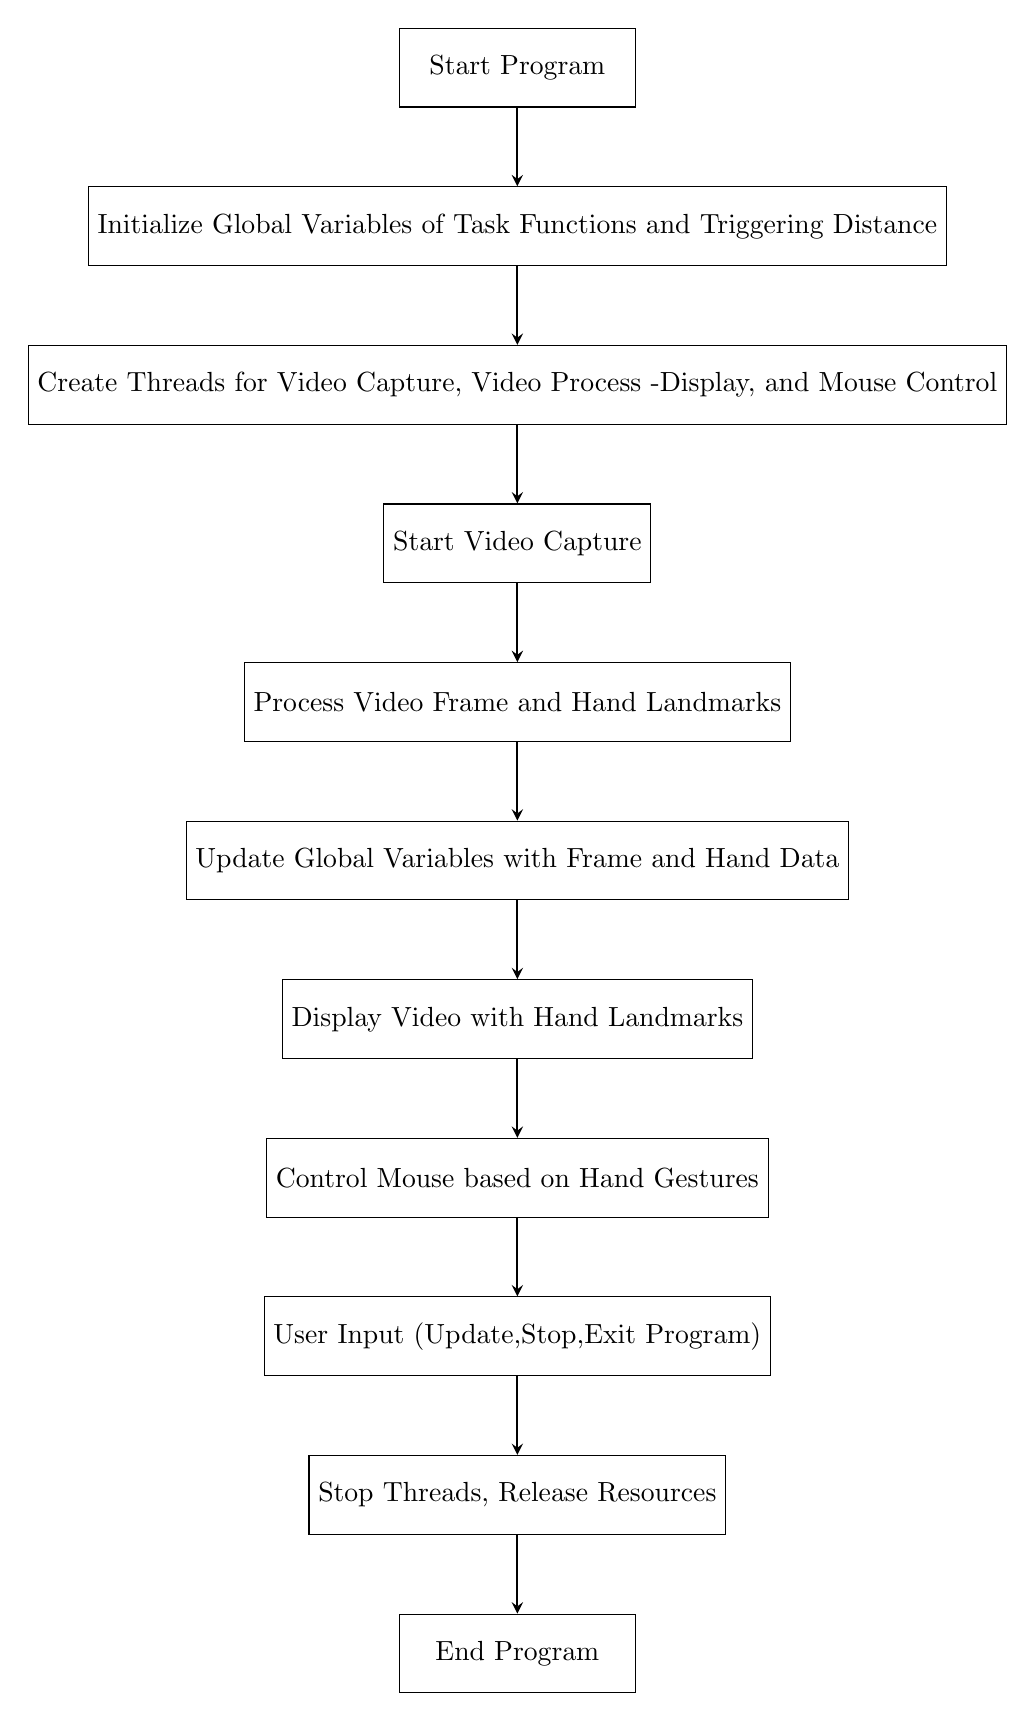
\begin{tikzpicture}[
    node distance=1cm,
    box/.style={draw, minimum width=3cm, minimum height=1cm, text centered},
    arrow/.style={thick,->,>=stealth}
]

\node (start) [box] {Start Program};
\node (init) [box, below=of start] {Initialize Global Variables of Task Functions and Triggering Distance};
\node (threads) [box, below=of init] {Create Threads for Video Capture, Video Process -Display, and Mouse Control};
\node (capture) [box, below=of threads] {Start Video Capture};
\node (process) [box, below=of capture] {Process Video Frame and Hand Landmarks};
\node (update) [box, below=of process] {Update Global Variables with Frame and Hand Data};
\node (display) [box, below=of update] {Display Video with Hand Landmarks};
\node (control) [box, below=of display] {Control Mouse based on Hand Gestures};
\node (input) [box, below=of control] {User Input (Update,Stop,Exit Program)};
\node (stop) [box, below=of input] {Stop Threads, Release Resources};
\node (end) [box, below=of stop] {End Program};

\draw [arrow] (start) -- (init);
\draw [arrow] (init) -- (threads);
\draw [arrow] (threads) -- (capture);
\draw [arrow] (capture) -- (process);

\draw [arrow] (process) -- (update);
\draw [arrow] (update) -- (display);
\draw [arrow] (display) -- (control);
\draw [arrow] (control) -- (input);
\draw [arrow] (input) -- (stop);
\draw [arrow] (stop) -- (end);

\end{tikzpicture}
		

		{\vfill \chapter*{\centering \vfill Chapter 3 \vfill}\vfill}
		\thispagestyle{empty}
		\newpage
		\label{Features of Virtual Mouse}
		\section{Features of Virtual Mouse }
		The program is being controlled by GUI; an application program has been developed for this purpose. Functionality are Listed below: 
		\begin{center}
Moving Cursor 

Left Click 

Right Click 

Scroll Up

Scroll Down 

Tab Change

Open Window Change 

Minimize all Tabs 

Collapse a Window 

Press Enter 

Open On-Screen keyboard 

Open File Manager

Screen Lock 

Some Game Controls 
		\end{center}
		\label{Function 1 ( Cursor Moving)}
		\subsection{Function 1 ( Cursor Moving)}
		Hand landmark 9 is used for moving the cursor as it is a centred as well as one of the stable node in human hand. Mouse pointer will move according to the movement of landmark 9.
\\ \\
		    \begin{tabular}{c c}
 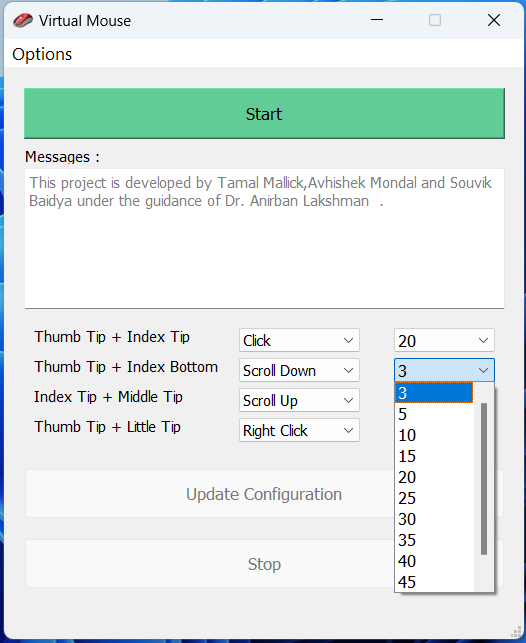
\includegraphics[width=0.4\textwidth]{soptions}&
 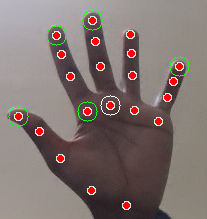
\includegraphics[width=0.4\textwidth]{action1} 
    \end{tabular}
		\label{Function 2 ( Click )}
		\subsection{Function 2 ( Click )}	Bringing hand landmarks 4 (Tip of the Thumb) and 8 (Tip of the Index Finger) within a certain distance(triggering distance) activates function 2 which perform mouse click (Left Click) operation. As most of the functions can be changed and updated at any moment of program runtime so kept it as a constant so that the virtual mouse can be operated efficiently .  
	\\ \\
		    \begin{tabular}{c c}
 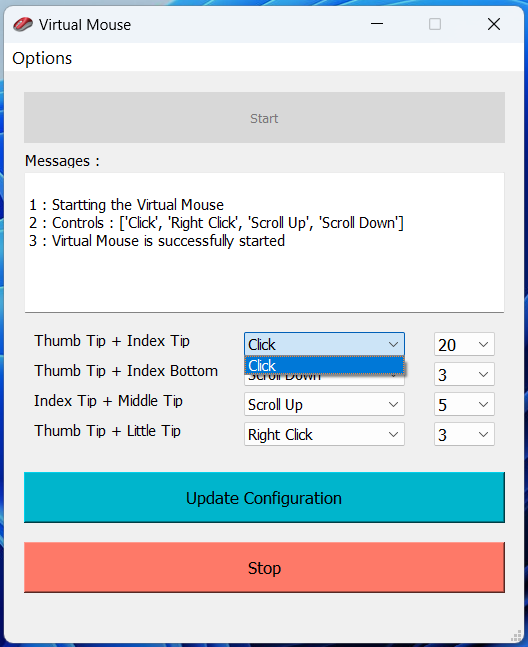
\includegraphics[width=0.4\textwidth]{action2f}&
 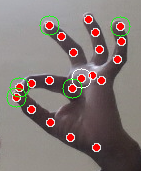
\includegraphics[width=0.4\textwidth]{action2} 
    \end{tabular}
    		\label{Function 3 ( Selectable )}
		\subsection{Function 3 ( Selectable )}	Bringing hand landmarks 4 (Tip of Thumb) and 5 (Bottom of the Index Finger) within a certain distance(triggering distance) activates function 3 which can be used to perform any one of the \textbf{Left Click ,Right Click ,Scroll Up,Scroll Down,Tab Change,Open Window Change,Minimize all Tabs,Open File Manager,Collapse a Window ,Press Enter ,Open On-Screen keyboard ,Screen Lock} any one of the task at a time. The \textbf{task} and \textbf{triggering distance} assigned to the function 3 \textbf{can be changed and updated at any moment of time using its user interface} and click method assigned to function 2 .This feature makes the virtual mouse highly dynamic and useful.
	\\ \\
		    \begin{tabular}{c c}
 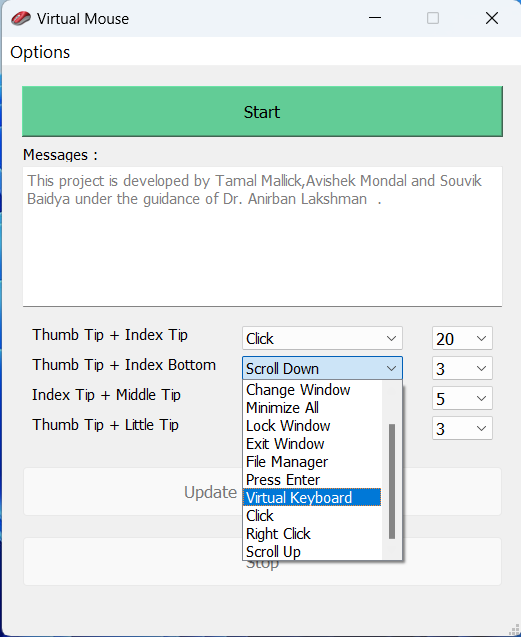
\includegraphics[width=0.4\textwidth]{action3f}&
 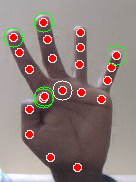
\includegraphics[width=0.4\textwidth]{action3} 
    \end{tabular}
    		\label{Function 4 ( Selectable )}
		\subsection{Function 4 ( Selectable )}Bringing hand landmarks 8 (Tip of the Index Finger) and 12 (Tip of the Middle Finger) within a certain distance(triggering distance) activates function 4 which can be used to perform any one of the \textbf{Left Click ,Right Click ,Scroll Up,Scroll Down,Open File Manager,Tab Change,Open Window Change,Minimize all Tabs,Collapse a Window ,Press Enter ,Open On-Screen keyboard ,Screen Lock} any one of the task at a time. The \textbf{task} and \textbf{triggering distance} assigned to the function 3 \textbf{can be changed and updated at any moment of time using its user interface} and click method assigned to function 2 .This feature makes the virtual mouse highly dynamic and useful.
	\\ \\
		    \begin{tabular}{c c}
 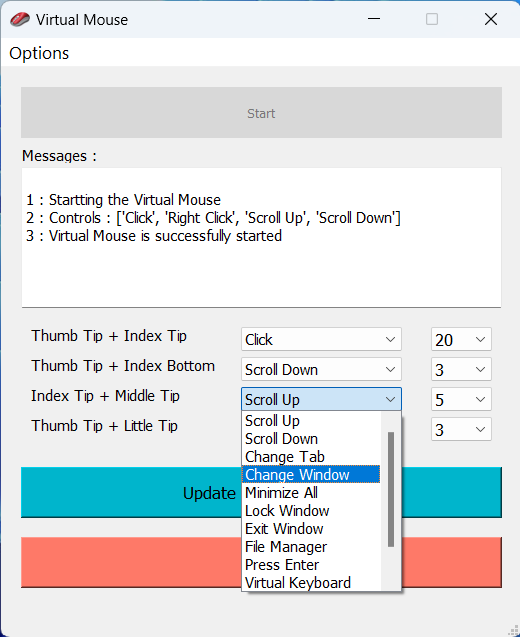
\includegraphics[width=0.4\textwidth]{action4f}&
 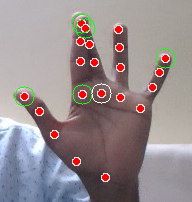
\includegraphics[width=0.4\textwidth]{action4} 
    \end{tabular}
    		\label{Function 5 ( Selectable )}
		\subsection{Function 5 ( Selectable )}Bringing hand landmarks 4 (Tip of Thumb) and 20 (Tip of the smallest Finger) within a certain distance(triggering distance) activates function 5 which can be used to perform any one of the \textbf{Left Click ,Right Click ,Scroll Up,Scroll Down,Open File Manager,Tab Change,Open Window Change,Minimize all Tabs,Collapse a Window ,Press Enter ,Open On-Screen keyboard ,Screen Lock} any one of the task at a time. The \textbf{task} and \textbf{triggering distance} assigned to the function 3 \textbf{can be changed and updated at any moment of time using its user interface} and click method assigned to function 2 .This feature makes the virtual mouse highly dynamic and useful. \\
		    \begin{tabular}{c c}
 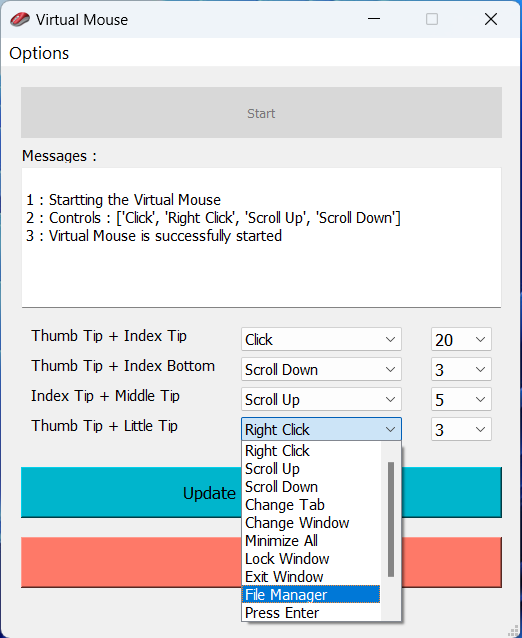
\includegraphics[width=0.35\textwidth]{action5f}&
 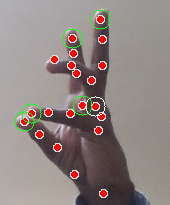
\includegraphics[width=0.35\textwidth]{action5} 
    \end{tabular}
		\label{Others}
		\subsection{Others} The program supports dynamic task execution, easily accommodating the addition of numerous actions like 'W,' 'S,' 'A,' 'D,' 'X,' 'R,' 'E,' and more for game control. It offers start, update, and stop options, and can be halted with \textbf{Shift + C}. Additionally, users can set triggering distances for functions 2 to 5 via the interface.
				\\ \\
				    \begin{tabular}{c c}
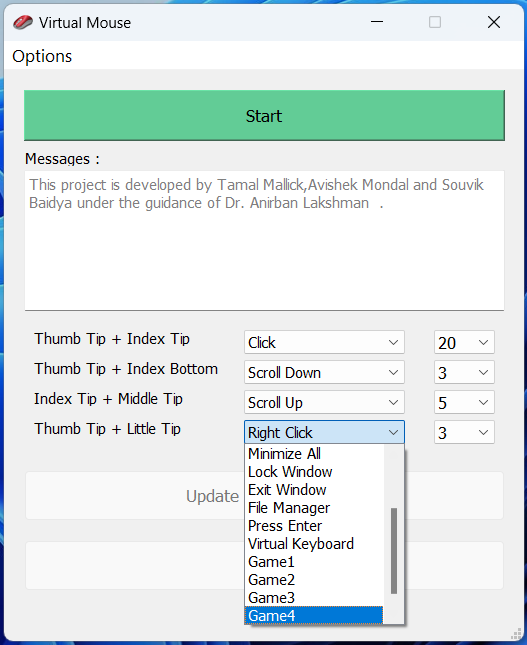
\includegraphics[width=0.35\textwidth]{goptions} & 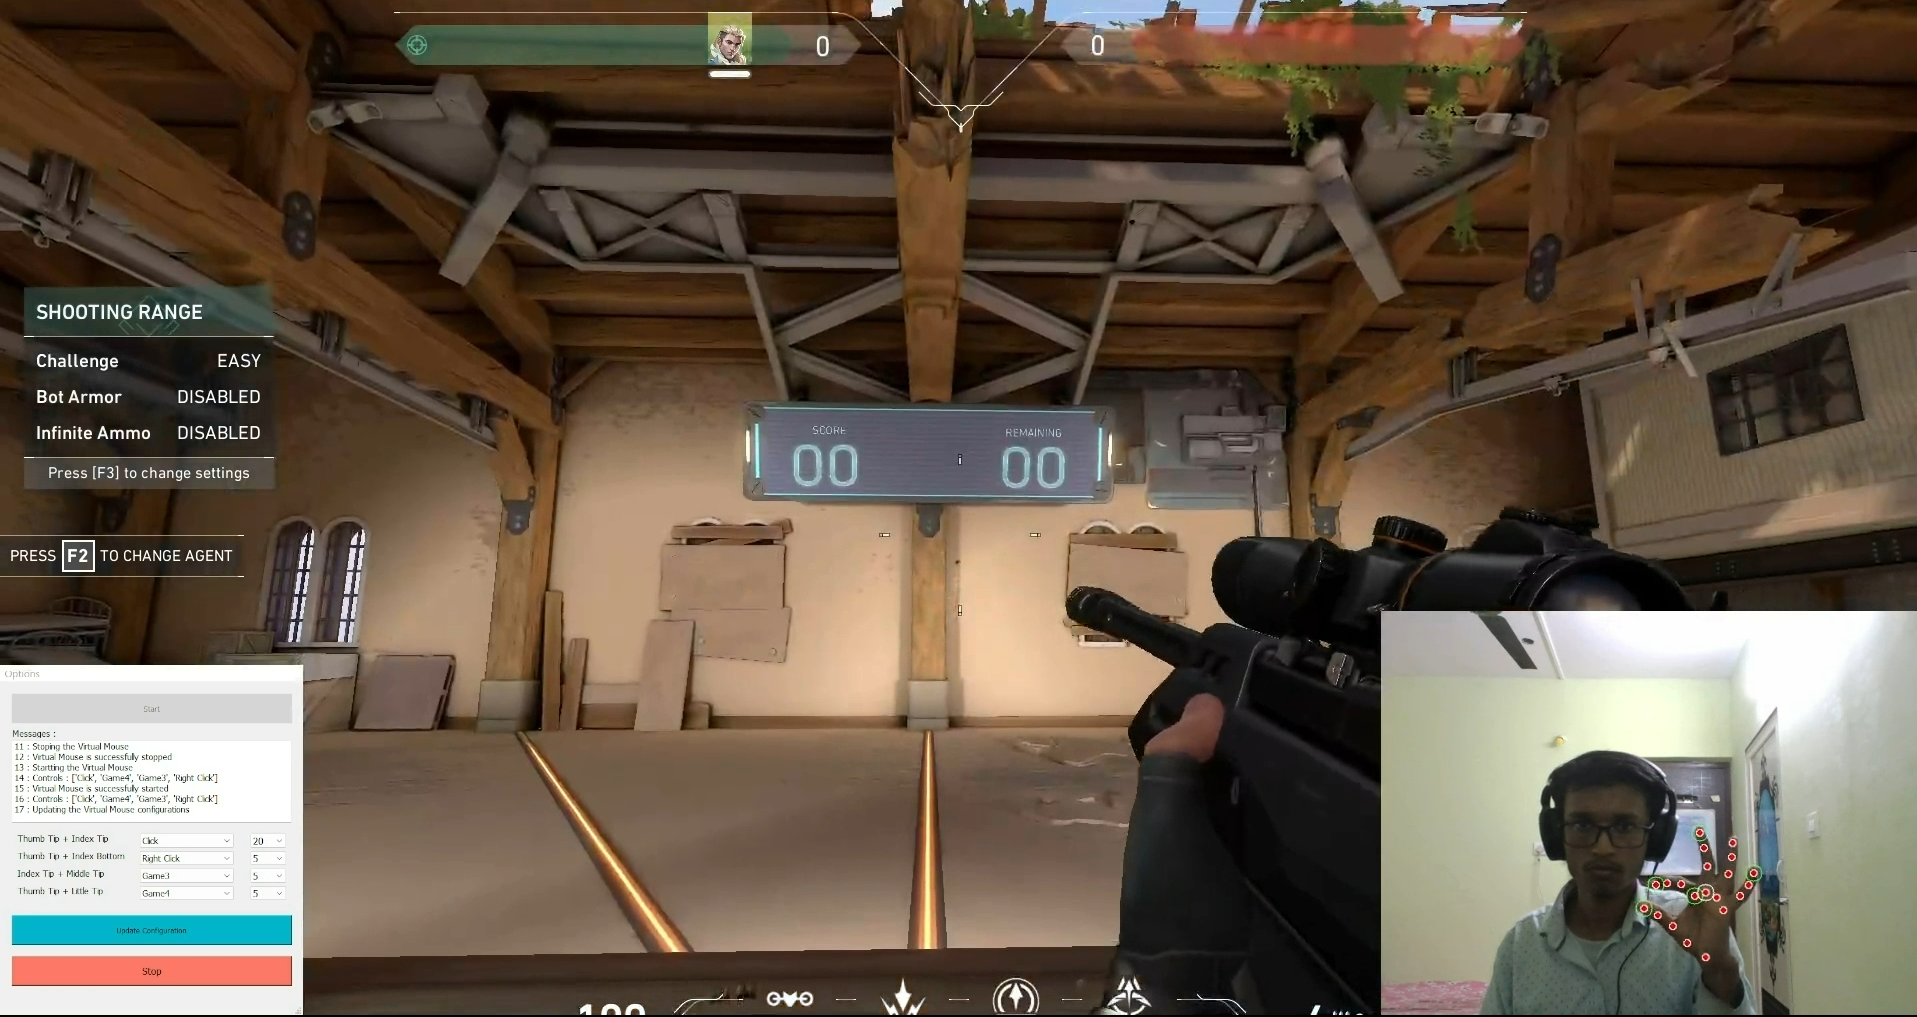
\includegraphics[width=0.6\textwidth]{gplay}
    \end{tabular} 
    \subsubsection{Gaming}
		In gaming, we are using Game mode 1 to 4 to perform activities like reloading and buying  guns,shooting,using in game utilities in a video game, for our testing we have used VALORANT . We can assign different functions to these game modes by changing the control keys in the game or in program itself.For more information please visit ,
		\begin{itemize}
    \item \url{https://youtu.be/2ky4_TPi58M}  or,
    \item \url{https://drive.google.com/drive/folders/1QC3p6UVEPqDbIh9Pla0QXFhP_69HhJ_O?usp=sharing}
\end{itemize}
 to access a video Example of Game playing using this Virtual Mouse Technology.
%		[\url{https://youtu.be/2ky4_TPi58M} or, \url{https://drive.google.com/drive/folders/1QC3p6UVEPqDbIh9Pla0QXFhP_69HhJ_O?usp=sharing}]

		%\linebreak https://youtu.be/2ky4_TPi58M
				{\vfill \chapter*{\centering \vfill Chapter 4 \vfill}\vfill}
				\thispagestyle{empty}
	\newpage
	\label{Performance Analysis}
	\section{Performance Analysis}{
		In the proposed AI virtual mouse system, the concept of advancing the Human-Computer interaction using computer vision is given. The hand gestures and fingertips detection have been tested in various luminous conditions and also been tested from various distance from the different distance and different hand gesture. The test was performed 25 times 8 rounds by each person total of three and this test has been done from different distance and different light condition. Each person tested,

 	\begin{itemize}
    \item \textbf{7 times in normal light condition} ( Far distance, near     distance, long distance), 
    \item \textbf{5 times in faint condition} ( Far distance, near distance, long distance), 
    \item \textbf{5 times in dark condition}(Far distance, near distance, long distance). 
\end{itemize}
	\label{Test Results of Functionalities}
	\subsection{Test Results of Functionalities}
	\begin{table}[h]
    \centering
    \begin{tabular}{|c|c|c|c|}
        \hline
        \textbf{Mouse Function} & \textbf{Success} & \textbf{Failure} & \textbf{Accuracy} \\
        \hline
        Mouse movement & 90 & 10 & 90\% \\
        \hline
        Left click & 80 & 20 & 80\% \\
        \hline
        Right click & 70 & 30 & 70\% \\
        \hline
        Scroll Down & 80 & 20 & 80\% \\
        \hline
        Scroll Up & 80 & 20 & 80\% \\
        \hline
        Others & 75 & 25 & 75\% \\
        \hline
    \end{tabular}
    \caption{Test Results of Functionalities}
    \label{tab:Test Results of Functionalities}
\end{table}
From the Table it can be seen proposed Virtual mouse system had achieved an accuracy of about 79%. From this accuracy of the proposed Virtual mouse, we come to know that the proposed mouse has performed well. 	
	}	
\newpage
	\label{Test Results in Different Conditions}
	\subsection{Test Results in Different Conditions}{
\begin{table}[h]
    \centering
    \begin{tabular}{|c|p{3cm}|p{1.9cm}|p{5cm}|c|c}
        \hline
        \textbf{Case Id} & \textbf{Scenario} & \textbf{Boundary Value} & \textbf{Expected Result} & \textbf{Result} \\
        \hline
        1 & Used in normal environment & 80\% & In normal environment Hand gesture can be recognized easily & Passed \\
        \hline
        2 & Used in Bright Light & 70\% & In bright brighter environment, software should work fine as it easily detects hand & Passed \\
        \hline
        3 & Used in Dark environment & 60\% & In a dark environment, it may not work properly & Passed \\
        \hline
        4 & Used at a near distance (15 cm) & 60\% & At short distance software should perform perfectly & Passed \\
        \hline
        5 & Used a far distance (35 cm) & 80\% & At this distance, software should perform fine & Passed \\
        \hline
        6 & Used further distance from camera & 75\% & Far distance, there will be some problem in detecting hand gesture & Passed \\
        \hline
    \end{tabular}
    \caption{Test Results in Different Conditions}
    \label{tab:Test Results in Different Conditions}
\end{table}
\thispagestyle{empty}
 \newpage
			{\vfill \chapter*{\centering \vfill Chapter 5 \vfill}\vfill}
		\thispagestyle{empty}
	
	\newpage
	\label{Conclusion and Future Scope}
	\section{Conclusion and Future Scope}
{
	\subsection{Conclusion}	The virtual mouse project successfully demonstrates the feasibility of using hand gestures as an alternative to traditional mouse input. The project effectively integrates OpenCV, Media Pipe, and PyAutoGUI to achieve real-time hand detection, tracking, and cursor control. The implemented features, including cursor movement, clicking, scrolling, and brightness/volume control, provide a versatile and intuitive user experience. 

The virtual mouse technology offers several advantages over traditional mouse input, including accessibility for individuals with disabilities, ergonomic benefits to reduce strain on wrists and hands, and portability for seamless transitions between devices. 	
	}
	\subsection{Future Scope}	The virtual mouse project presents promising avenues for future research and development: 

		\begin{itemize}
		
    \item Enhance Hand Gesture Recognition: Continuously improve the accuracy and robustness of hand gesture recognition, particularly for complex and subtle gestures.
    
    \item Expand Feature Set: Incorporate additional features, such as gesture-based commands, application-specific interactions, and support for multiple users. 
    
    \item Explore Integration with VR/AR: Investigate the integration of virtual mouse technology with virtual reality (VR) and augmented reality (AR) environments for enhanced user immersion and interaction. 
    \item Mobile Application Development: Develop a mobile application version of the virtual mouse, leveraging smartphone cameras and gesture recognition capabilities. 
    \item Enhanced Immersive Experiences: Virtual mouse technology has the potential to enhance gaming experiences by offering more immersive and interactive gameplay. Players can use hand gestures or motions to control elements within the game, providing a more natural and engaging gaming environment.
    \item Real-world Implementation and Testing: Conduct extensive real-world testing and user evaluation to gather feedback and refine the virtual mouse technology for practical applications. 
	
	\end{itemize}

	
	The virtual mouse technology holds immense potential to revolutionize human-computer interaction, making computers more accessible, ergonomic, and intuitive for users worldwide. As technology continues to evolve, we can expect to see its adoption in various domains, from personal computing to healthcare, education, and entertainment. 
	\newpage
				{\vfill \chapter*{\centering \vfill Chapter 6 \vfill}\vfill}
		\thispagestyle{empty}
		\newpage
	\section{References}
	
\end{document}